\documentclass[a4paper, 12pt]{article}
\usepackage{graphicx}
\usepackage[spanish,es-tabla]{babel} %Para que lo que pinte latex automáticamente lo haga en español
\usepackage[hidelinks]{hyperref}
\usepackage{tabularx}
\renewcommand{\shorthandsspanish}{}
\renewcommand{\refname}{Bibliografía}
\usepackage{float}
\usepackage[table]{xcolor}
\pretolerance=10000
\usepackage[shortlabels]{enumitem}
\usepackage[autostyle]{csquotes} 

\begin{document}

%%%%%%%%%%%%%%%%%%%%%%%%%%%%%%%%%%%%%%%%%%%%%%%%%%%%%%%%%%%%%%%%%%%%%%%
% PORTADA
%%%%%%%%%%%%%%%%%%%%%%%%%%%%%%%%%%%%%%%%%%%%%%%%%%%%%%%%%%%%%%%%%%%%%%%
\begin{titlepage}

	\begin{flushright}
		
\includegraphics[scale=0.25]{img/logo.png}
	\end{flushright}

\vspace{3cm}
\begin{center}
{\Large
Tipología y ciclo de vida de los datos.\\


Máster Universitario en Ciencia de Datos

}
\end{center}
\vspace{3.8cm}
\begin{flushleft}
{\Large
Práctica 1:}\\ 
\vspace{0.20cm}
{\Large
{\itshape Scraper} a una web inmobiliaria.
\\ }

\vspace{1.8cm}

\textbf{Autores:} 
\begin{itemize}
	\item Andrea Giralt Castellano
	\item Manuel Fernández Álvarez
\end{itemize}

\textbf{Profesor:} Jose Moreira Sanchez \\ 

\end{flushleft}

\begin{flushleft}
Lunes, 8 de noviembre de 2021
\end{flushleft}

\end{titlepage}

%%%%%%%%%%%%%%%%%
% PÁGINA EN BLANCO
\newpage
\mbox{}
\thispagestyle{empty} % para que no se numere esta pagina
\clearpage

%%%%%%%%%%%%%%%%%
% SECCIONES

\tableofcontents
\clearpage %Salto de página.

\section{Contexto}

En este proyecto se ha decidido extraer información de la web \href{https://www.pisos.com} {\textcolor{cyan}{\underline{{\itshape pisos.com}}}}. Esta plataforma, donde el producto a comercializar son inmuebles, permite unir tanto a los compradores como a los vendedores. Es importante destacar que los anunciantes pueden ser tanto particulares como inmobiliarias. 

En un entorno donde conseguir un comprador es complicado, utilizar plataformas donde poder anunciarte de forma gratuita es primordial. Por esta razón, muchos particulares o inmobiliarias utilizan estas plataformas para publicitarse y darse a conocer utilizándolas, también, para poder analizar los precios de mercado con el fin de dar un precio competitivo respecto al resto de inmuebles. 

Es por eso que este análisis permitirá tanto a particulares como a los profesionales de inmobiliaria a:
\begin{itemize}
	\item Hacer estudios para identificar las zonas más caras o que están en auge.
	\item Detectar gangas o viviendas que están muy por encima del precio del mercado.
	\item Estimar el precio de una vivienda, dada sus características.
	\item Análisis de posibles variables estacionales.
	\item Análisis de un posible incremento en el precio si el anunciante es una inmobiliaria.
	\item Análisis de la posible influencia del paro en el precio de un inmueble.
\end{itemize}


Por otro lado, es importante destacar que nuestros datos no son de carácter personal, ya que solamente tenemos información de los inmuebles y no de las personas a las cuales pertenecen, luego cumplimos la RGPD. 

Aun así, si tuviésemos datos de carácter personal, podríamos utilizarlos y cumplir con la RGDP, siempre y cuando tuviésemos el consentimiento del usuario poseedor de los datos.

Por último, con el fin de realizar un estudio de posible influencia del paro al precio de la vivienda, se procesado empleando un {\itshape spider}, el último csv disponible en la URL:
\href{ https://datos.gob.es/es/catalogo/ea0021425-paro-registrado-por-municipios} {\textcolor{cyan}{\underline{{\itshape datos.gob.es}}}} el cual, actualmente, recoge los datos de paro por municipio a nivel estatal hasta septiembre de 2021.

\section{Título}

Análisis del sector inmobiliario en Mallorca.

\section{Descripción del {\itshape dataset}}

El dataset, por tanto, recoge los datos más relevantes que pueden influir en el precio de un inmueble. En este dataset, se presentan los datos obtenidos de una descarga puntual de un día, de los inmuebles de Mallorca. Las unidades del precio de la vivienda son en euros. Hay que tener en cuenta que los datos no han pasado por ningún proceso de limpieza, por lo que este proceso se realizará en la práctica siguiente. El formato final del dataset es un fichero CSV.

\section{Representación gráfica}

Como podemos ver en la imagen, existen dos tipos de publicitantes, las personas físicas, llamadas vendedores en la imagen, o las inmobiliarias. Ambos pueden poner un anuncio de forma gratuita en \href{https://www.pisos.com} {\textcolor{cyan}{\underline{{\itshape pisos.com}}}} sobre un inmueble. Por otro lado, existe la posibilidad de comprar anuncios clasificados, y es de aquí de donde \href{https://www.pisos.com} {\textcolor{cyan}{\underline{{\itshape pisos.com}}}} obtienen sus ganancias. Estos anuncios, son destacados en la web por encima de otros e incluso son propuestos a aquellos compradores que por las características del inmueble cumplan sus requisitos.

\begin{figure}[H]
	\centering
	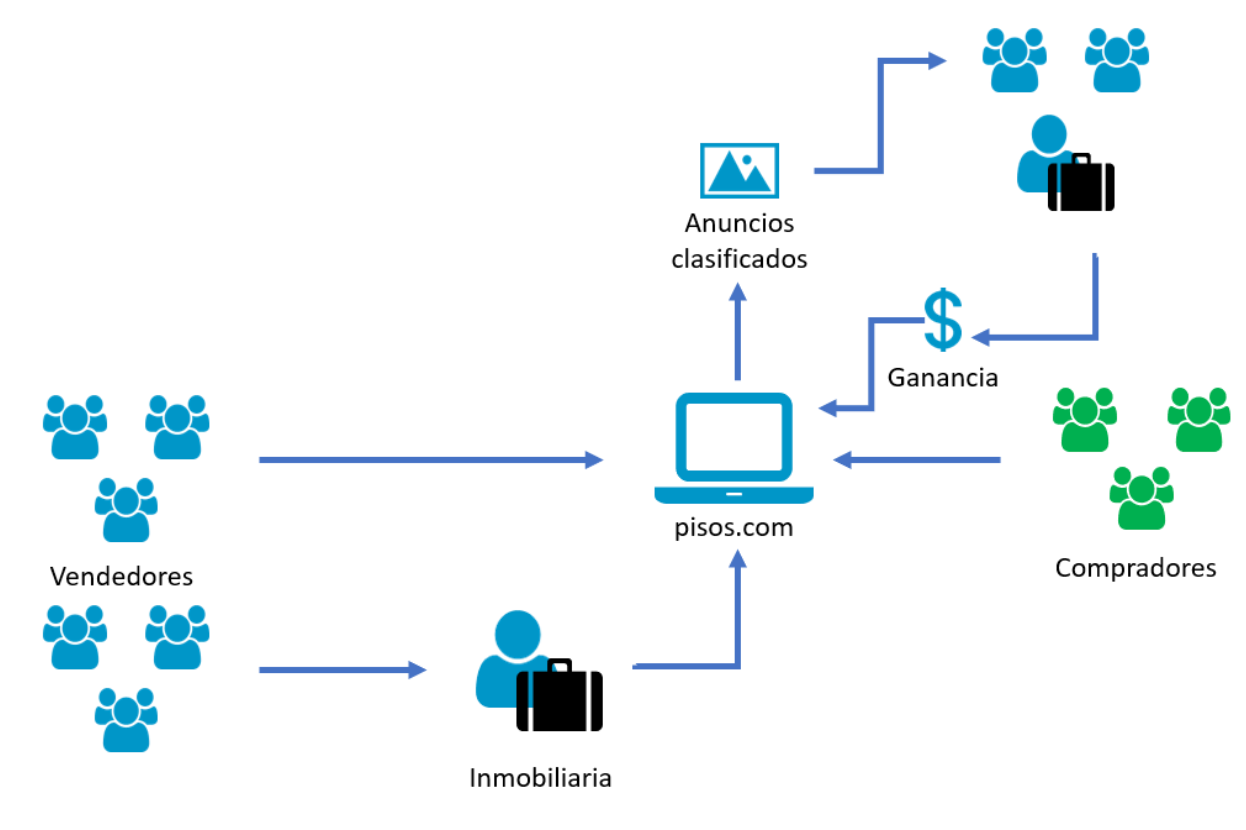
\includegraphics[width=0.7\linewidth]{img/screenshot007}
	\caption{Representación gráfica}
	\label{fig:screenshot007}
\end{figure}

\section{Contenido}

Los datos descargados se han obtenido en un día puntual, obteniendo un total de 5736 anuncios.

\begin{itemize}
	\item \textbf{{\itshape id}}: Identificador del anuncio en la web.
	\item \textbf{{\itshape type}}: Tipo de vivienda (Piso, Chalet, Apartamento…)
	\item \textbf{{\itshape title}}: Título del anuncio.
	\item \textbf{{\itshape description}}: Breve descripción del anuncio
	\item \textbf{{\itshape town}}: Municipio
	\item \textbf{{\itshape zone}}: Localidad
	\item \textbf{{\itshape price}}: Precio de la vivienda
	\item \textbf{{\itshape surface}}: Superficie en m2
	\item \textbf{{\itshape rooms}}: Número de habitaciones
	\item \textbf{{\itshape bathrooms}}: Números de baños
	\item \textbf{{\itshape floor}}: Planta donde se localiza el inmueble
	\item \textbf{{\itshape longitude}}: Coordenada longitud.
	\item \textbf{{\itshape latitude}}: Coordenada latitud.
	\item \textbf{{\itshape url}}: Enlace al anuncio.
	\item \textbf{{\itshape exact\_position}}: Si las coordenadas corresponden a una localización exacta.
	\item \textbf{{\itshape recently\_date}}: Fecha de publicación
	\item \textbf{{\itshape is\_promo}}: Si es una promoción.
	\item \textbf{{\itshape image\_url}}: Foto principal del inmueble.
	\item \textbf{{\itshape owner\_name}}: Nombre del publicador del anuncio.
	\item \textbf{{\itshape old\_price}}: Si ha habido una rebaja, correspondría al precio anterior.	
\end{itemize}

Por otro lado, se ha obtenido la siguiente información relativa al paro por municipio de Mallorca.

\begin{itemize}
	\item \textbf{Código Municipio}: Código postal del municipio.
	\item \textbf{Municipio}: Nombre del municipio.
	\item \textbf{total Paro Registrado}: Número total de parados.
	\item \textbf{Paro hombre edad $<$ 25}: Total de hombres parados menores de 25 años.
	\item \textbf{Paro hombre edad 25 - 45 }: Total de hombres parados entre 25 y 45 años.
	\item \textbf{Paro hombre edad $>$=45 }: Total de hombres parados mayores de 45 años.	
	\item \textbf{Paro mujer edad $<$ 25}: Total de mujeres paradas menores de 25 años.
	\item \textbf{Paro mujer edad 25-45 }: Total de mujeres paradas entre 25 y 45 años.
	\item \textbf{Paro mujer edad $<$=45 }: Total de mujeres paradas mayores de 45 años.	
	\item \textbf{Paro Agricultura }: Total de parados en el sector de la agricultura.
	\item \textbf{Paro Industria }: Total de parados en el sector de la industria.
	\item \textbf{Paro Construcción}: Total de parados en el sector de la construcción.
	\item \textbf{Paro Servicios}: Total de parados en el sector de servicios.
	\item \textbf{Paro Sin empleo Anterior}: Total de parados que no han tenido empleo con anterioridad.
	
\end{itemize}

Cómo se ya se ha comentario con anterioridad, los datos no han pasado por ningún proceso de limpieza, será en una segunda parte cuando se realizará la limpieza y se enlazará la información obtenida del portal inmobiliario, con el paro por municipio.

Los datos fueron recogidos a través de {\itshape web scraping} en lenguaje {\itshape python} sobre la página web: \href{https://www.pisos.com} {\textcolor{cyan}{\underline{{\itshape pisos.com}}}}. Como se ha indicado previamente, los datos extraídos se han guardado en un fichero CSV. Por lo tanto, para realizar este proyecto, se han seguido los siguientes pasos:
\begin{enumerate}
	
	\item Al tratarse de un equipo, aunque solo de dos personas, hemos empleado \href{https://www.trello.com} {\textcolor{cyan}{\underline{{\itshape trello.com}}}} para gestionar las tareas que se tenían que realizar.
	
	\begin{figure}[H]
		\centering
		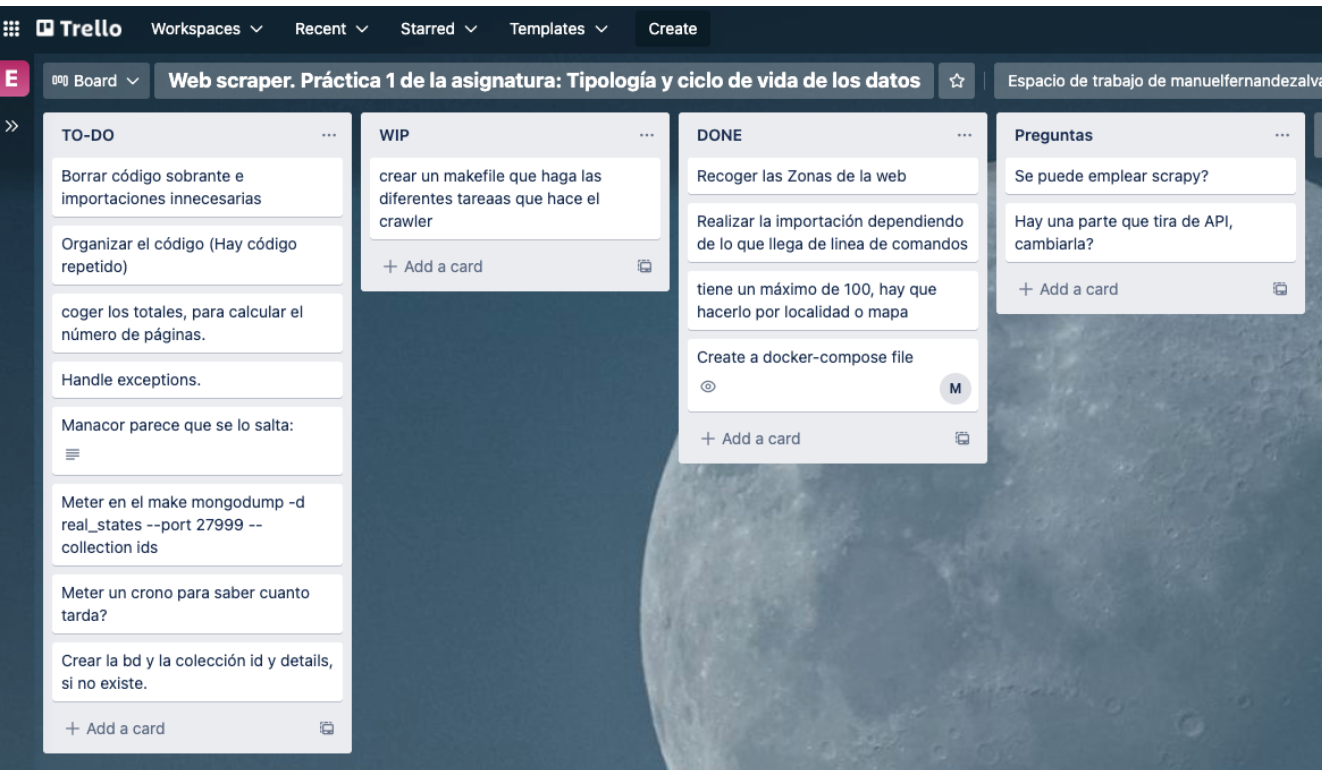
\includegraphics[width=0.7\linewidth]{img/screenshot008}
		\caption{Imagen del panel {\itshape trello}}
		\label{fig:screenshot008}
	\end{figure}
	\item Para proceder con el {\itshape scraping}, hemos entrado en la web de pisos.com, seleccionando "Islas Baleares", ya que nuestro análisis será exclusivamente de la isla de Mallorca.
	
	\begin{figure}[H]
		\centering
		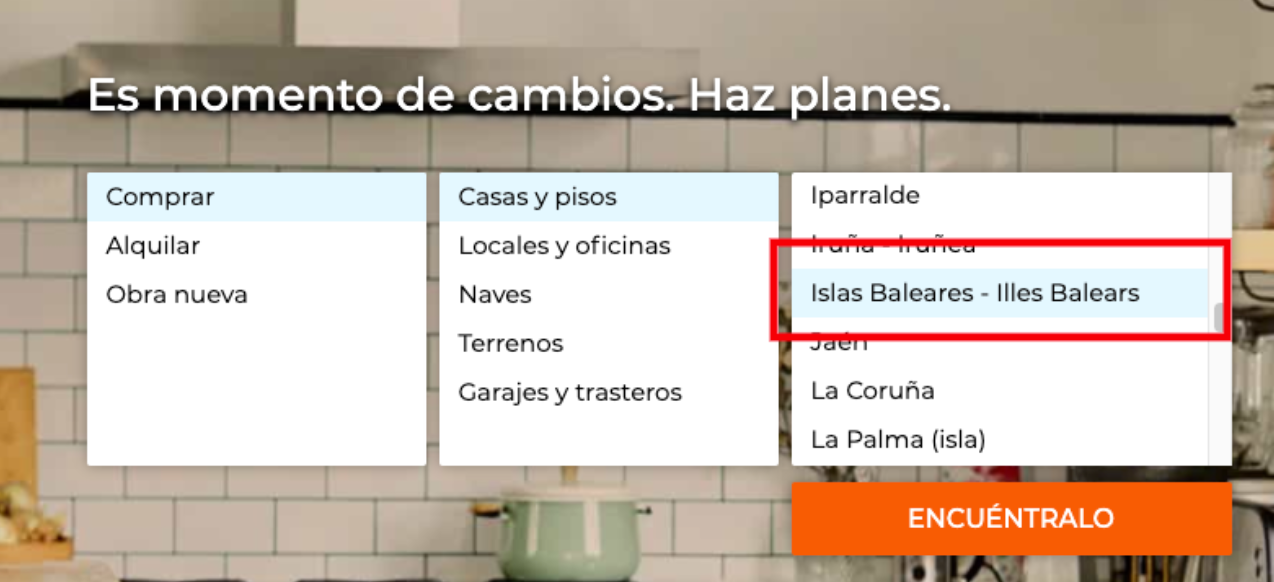
\includegraphics[width=0.7\linewidth]{img/screenshot009}
		\caption{Página de selección de provincia}
		\label{fig:screenshot009}
	\end{figure}
	
	
	\item A continuación, seleccionamos Mallorca:
	
	\begin{figure}[H]
		\centering
		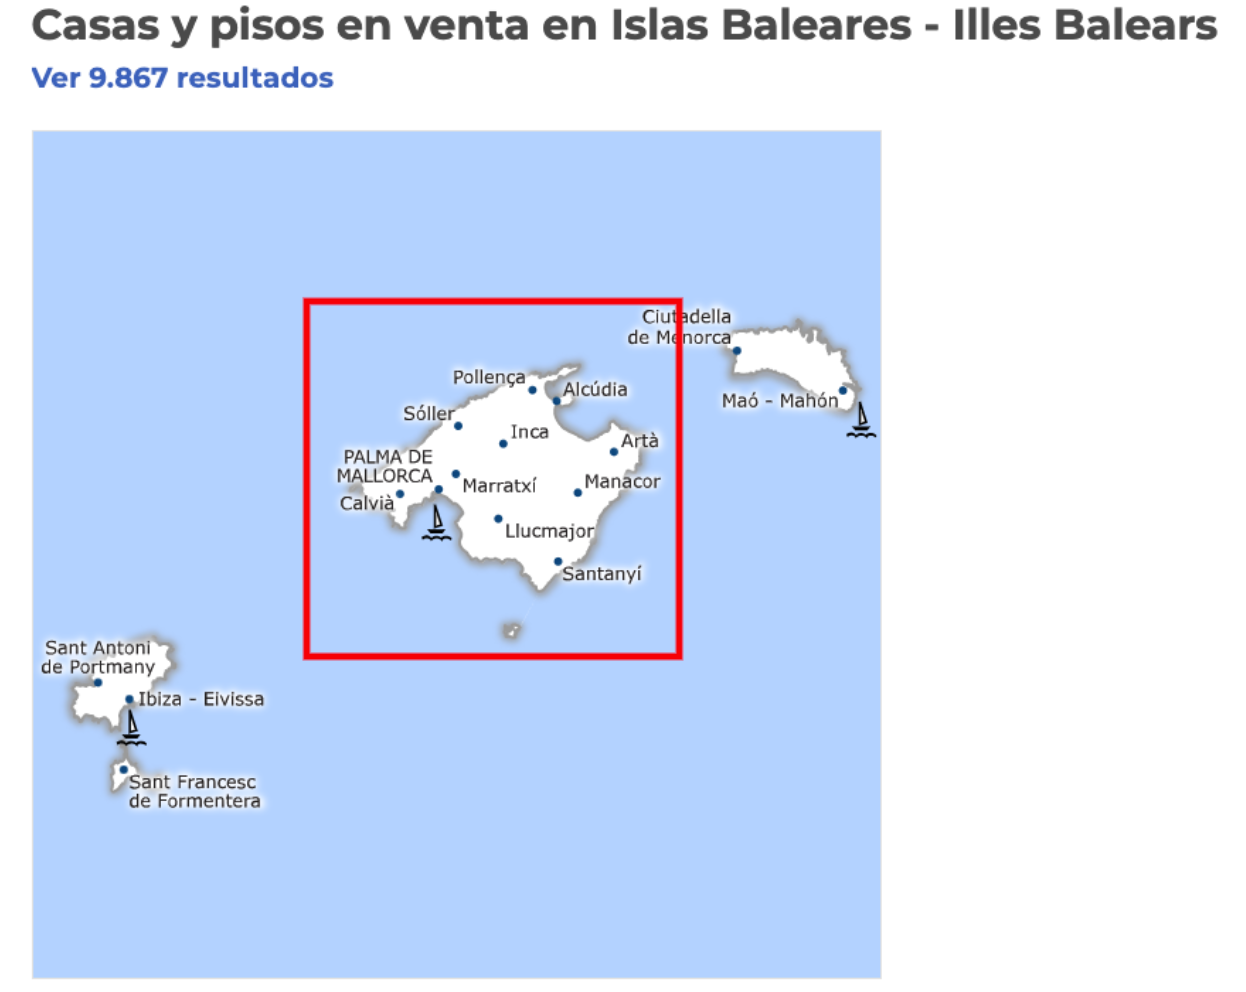
\includegraphics[width=0.7\linewidth]{img/screenshot010}
		\caption{Selección de Mallorca en el mapa}
		\label{fig:screenshot010}
	\end{figure}

	\item Como la web solo permite llegar hasta \underline{100 páginas en las búsquedas}, decidimos parsear por municipio en lugar de la isla entera.

	\begin{figure}[H]
		\centering
		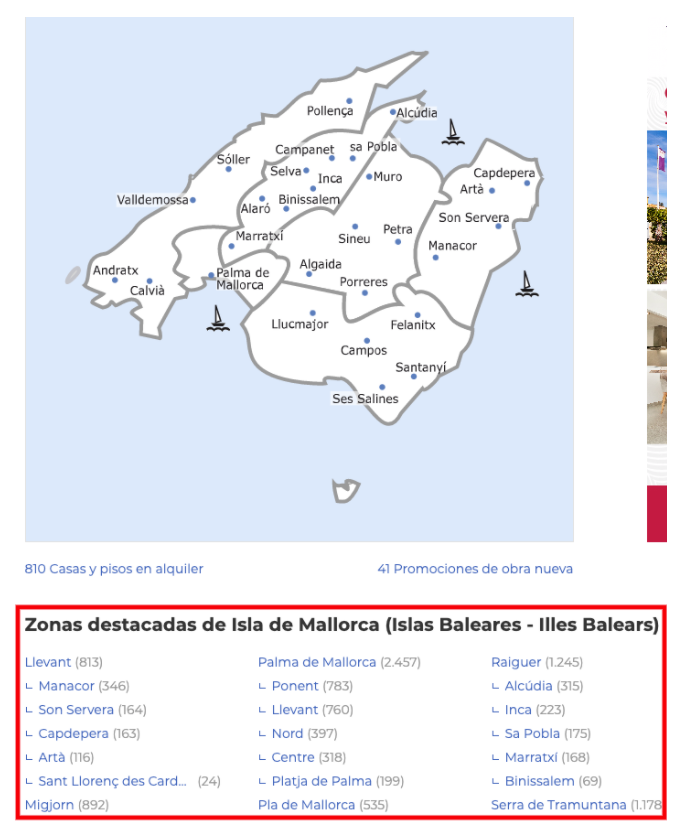
\includegraphics[width=0.7\linewidth]{img/screenshot011}
		\caption{Apartado con el listado de municipios}
		\label{fig:screenshot011}
	\end{figure}
	
	Por lo tanto, parseamos los enlaces y los totales (en cada página de búsqueda hay 30 anuncios).  Lo descargamos en un csv, para que el siguiente {\itshape spider} pueda hacer uso de él. (zones.py)
	
	\begin{figure}[H]
		\centering
		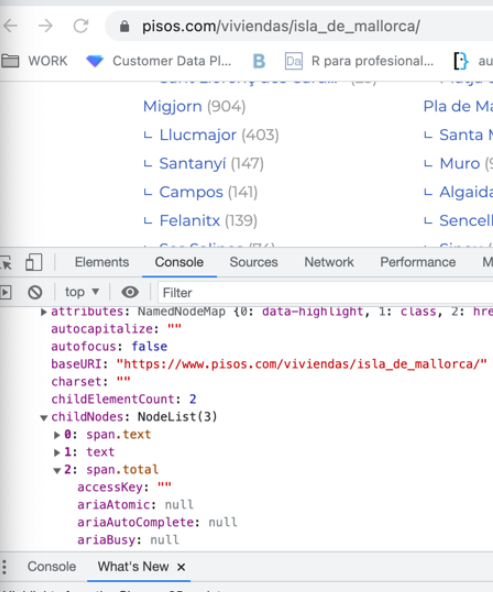
\includegraphics[width=0.7\linewidth]{img/screenshot012}
		\caption{Extracción de enlaces usando la consola}
		\label{fig:screenshot012}
	\end{figure}
	
	\item Vistamos los enlaces obtenidos en el paso anterior y vamos parseando por página:
	
	\begin{figure}[H]
		\centering
		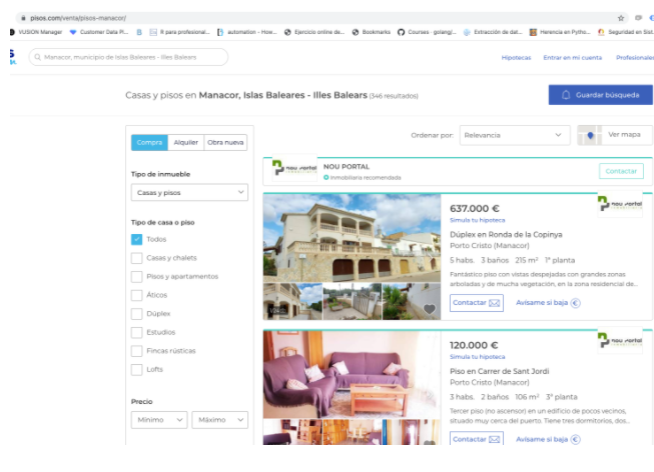
\includegraphics[width=0.7\linewidth]{img/screenshot013}
		\caption{Listado de anuncios, paginado, de un municipio.}
		\label{fig:screenshot013}
	\end{figure}
	
	\begin{figure}[H]
		\centering
		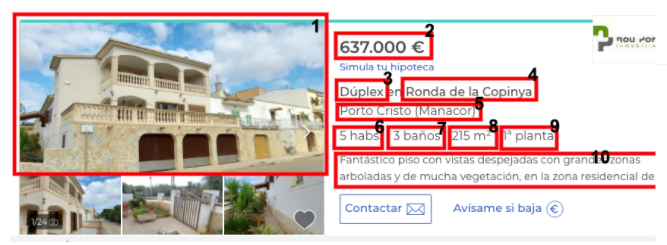
\includegraphics[width=0.7\linewidth]{img/screenshot015}
		\caption{Información extraída de las fichas de los inmuebles.}
		\label{fig:screenshot015}
	\end{figure}
	
	\item De estos listados (Figura \ref{fig:screenshot015}) nos descargamos la información previamente comentada:
		\begin{enumerate}[1.]
			\item Imagen principal del anuncio.
			\item Precio de la vivienda.
			\item Tipo de vivienda.
			\item Título
			\item Municipio/Localidad.
			\item Número de habitaciones.
			\item Número de baños.
			\item Superficie de la vivienda.
			\item Planta
			\item Breve descripción del anuncio.			
		\end{enumerate}

	Para procesar los campos de la ficha del anuncio, no solo hemos empleado selectores CSS3, también hemos hecho uso de expresiones regulares, como por ejemplo, para extraer el tipo de vivienda.
	
	\item  Esta información la hemos guardado en una base de datos NoSQL MongoDB, para después completarla con llamadas a una API en un tercer paso.
	
	\begin{figure}[H]
		\centering
		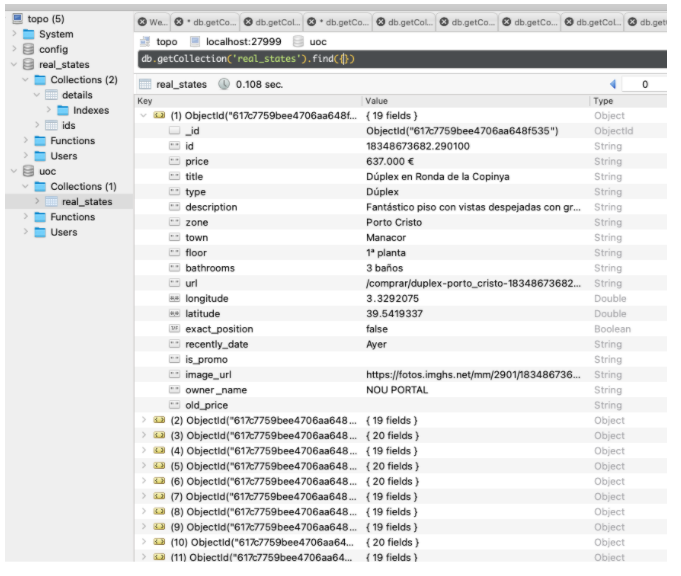
\includegraphics[width=0.7\linewidth]{img/screenshot016}
		\caption{Colección Mongo con la información básica}
		\label{fig:screenshot016}
	\end{figure}
	
	\item Por otro lado, nos dimos cuenta que en el mapa que contiene los anuncios, se construía a través de llamadas a una API.
	
	\begin{figure}[H]
		\centering
		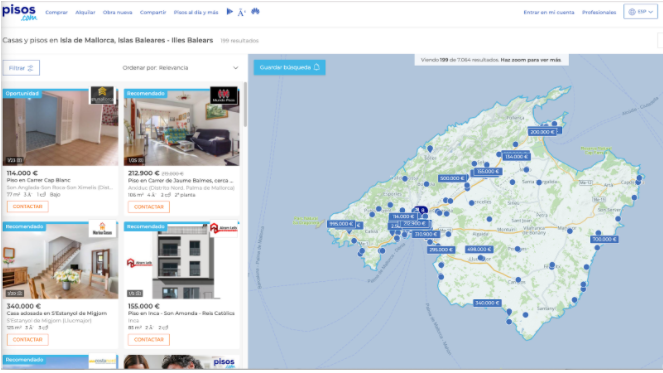
\includegraphics[width=0.7\linewidth]{img/screenshot017}
		\caption{Mapa interactivo de Mallorca}
		\label{fig:screenshot017}
	\end{figure}
	
	\begin{figure}[H]
		\centering
		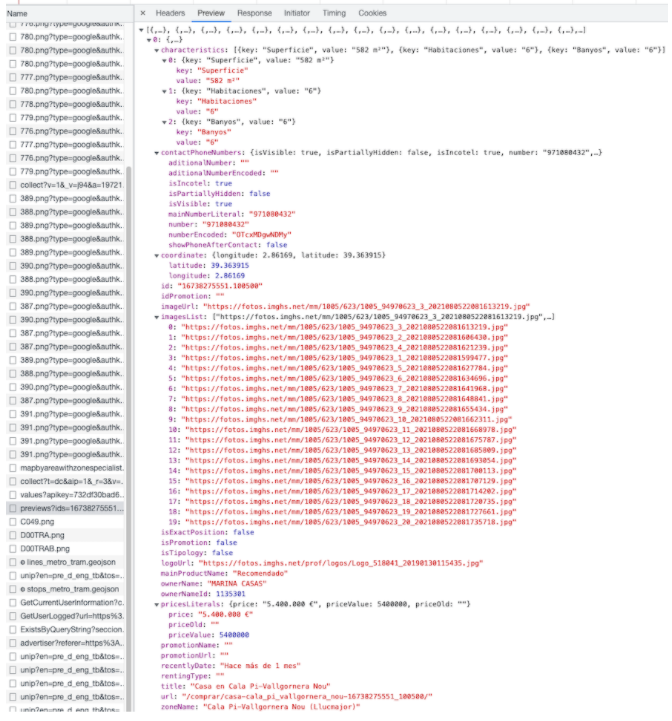
\includegraphics[width=0.7\linewidth]{img/screenshot018}
		\caption{Inspección de una llamada a la API}
		\label{fig:screenshot018}
	\end{figure}
	
	Con el fin de recolectar la información, hemos completado la información obtenida de las fichas de los anuncios con el resultado de llamar a esta API.
	
	Para poder llamar a la API, tenemos que emplear una cookie y una api-key asociada a ella, por lo que nos vimos en la obligación de añadir esta información a la cabeceras de las solicitudes.
	
	Completamos la información obtenida de la ficha del producto, con los siguientes campos: {\itshape url, longitude, latitude, exact\_position, recently\_date, is\_promo, image\_url, owner\_name, old\_price.}
	
	Por nuestra experiencia, sabíamos que, normalmente, las APIs, en la raíz, disponen de ayuda, por lo que descubrimos que, visitando la raíz, podíamos ver los distintos {\itshape endpoints} de los que disponen en la web, tal y como podemos ver en la siguiente imagen:
	
	\begin{figure}[H]
		\centering
		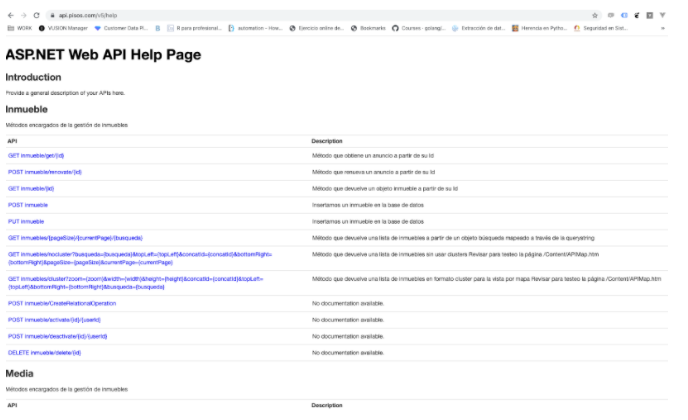
\includegraphics[width=0.7\linewidth]{img/screenshot019}
		\caption{Documentación de la API}
		\label{fig:screenshot019}
	\end{figure}
	
	Después de probar varios {\itshape endpoints}, nos dimos cuenta de que, a parte de carecer de documentación, muchos de ellos no funcionaban.
	
	\item Por último, con el fin de realizar un análisis de posible correlación del paro de un municipio con el precio de las viviendas, realizamos un procesado de la \href{https://datos.gob.es/es/catalogo/ea0021425-paro-registrado-por-municipios} {\textcolor{cyan}{\underline{{\itshape web del paro}}}}, extrayendo información de paro por municipio del país.
	
	\begin{figure}[H]
		\centering
		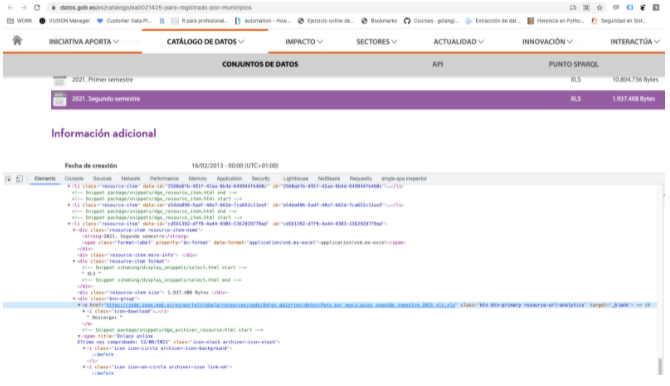
\includegraphics[width=0.7\linewidth]{img/screenshot020}
		\caption{Inspeccionando web de gob.es}
		\label{fig:screenshot020}
	\end{figure}
	
	Previsualizamos el contenido del excel descargado, para que sea más sencillo el procesado.
	
	\begin{figure}[H]
		\centering
		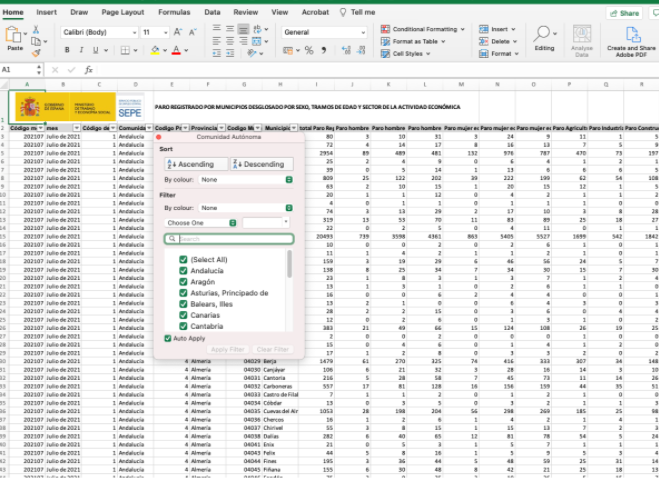
\includegraphics[width=0.7\linewidth]{img/screenshot021}
		\caption{Previsualización excel de gob.es}
		\label{fig:screenshot021}
	\end{figure}
	
	Echamos un vistazo a la información de la que disponemos para Baleares.
	
	\begin{figure}[H]
		\centering
		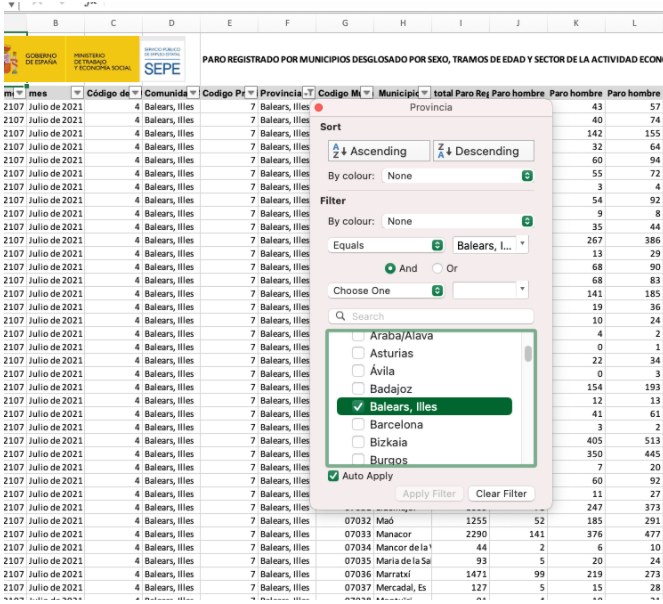
\includegraphics[width=0.7\linewidth]{img/screenshot022}
		\caption{Filtrado de excel por Baleares}
		\label{fig:screenshot022}
	\end{figure}
	
	Como estamos más acostumbrados a leer CSVs desde un {\itshape jupyter notebook}, abrimos uno para extraer la información que necesitamos del excel y después pasar el código resultante al {\itshape script} con los {\itshape spiders}.
	
	\begin{figure}[H]
		\centering
		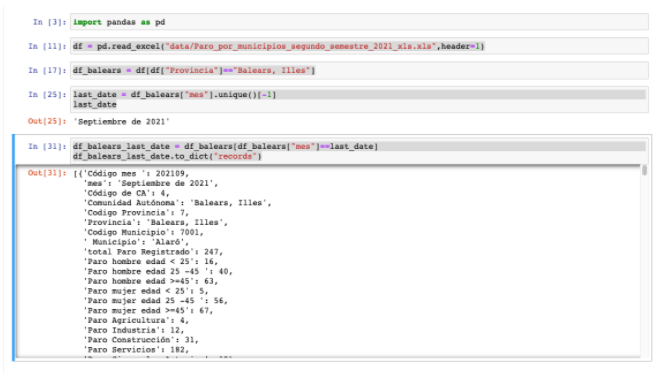
\includegraphics[width=0.7\linewidth]{img/screenshot023}
		\caption{Hoja {\itshape jupyter} para hacer las pruebas}
		\label{fig:screenshot023}
	\end{figure}
	
	Con el script, almacenamos la información en la base de datos NoSQL, en la colección "{\itshape unemployment}".
	
	\begin{figure}[H]
		\centering
		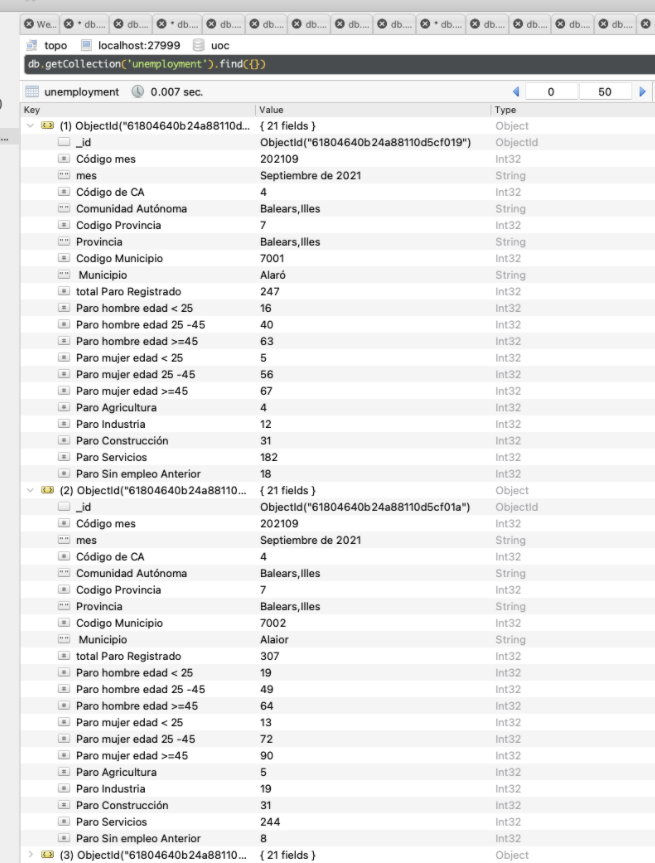
\includegraphics[width=0.7\linewidth]{img/screenshot024}
		\caption{Colección unemployment}
		\label{fig:screenshot024}
	\end{figure}
	
\end{enumerate}

\section{Agradecimientos}

Queremos agradecer la elaboración de este proyecto a nuestras familias, por entendernos y apoyarnos en la lucha para ser mejores profesionales. Por otro lado, nos gustaría agradecer a las personas encargadas de elaborar la diferente documentación que hemos ido consultando durante este proyecto, sin ellos hubiese sido mucho más complicado. Por último, agradecer también a la web pisos.com, por dejarnos acceder a sus anuncios y conseguir, así, los datos para la realización del proyecto.

\section{Inspiración}

El interés en analizar este conjunto de datos es poder analizar un sector de interés público, en el cual se puedan identificar posibles oportunidades de inversión o, incluso, de estafa. Se debe destacar que el sector inmobiliario es un sector muy cambiante e influenciable, por lo que como posible mejora sería interesante tener un histórico de todos los inmuebles que se han puesto a la venta a lo largo del tiempo. Además, también sería interesante hacer el estudio a nivel estatal y no solo de Mallorca.\\
Por otro lado, en este análisis, se pretende responder a las siguientes cuestiones:
\begin{itemize}
\item ¿Cuáles son las características de las viviendas más caras? ¿Y de las más baratas?
\item ¿Cuáles son las viviendas que, por sus características, están por debajo del precio medio del mercado? ¿Y las que están por encima?
\item ¿Cuál es la zona más barata donde comprar una vivienda? ¿Y la más cara?
\item ¿Cuáles son las variables estacionales de nuestro dataset?
\item ¿Son los precios de los inmuebles más caros si el anunciante es una inmobiliaria?
\item ¿Podemos estimar el precio de la vivienda con los datos obtenidos?
\item ¿El paro del municipio es una variable que afecta al precio medio por municipio de los inmuebles?
\end{itemize}

\section{Licencia}

Para nuestro conjunto de datos, escogeremos la licencia {\itshape CC BY-SA 4.0 License}, ya que permite proveerse del nombre del creador del {\itshape dataset} generado, indicando los posibles cambios realizados. Así, permite reconocer el trabajo de terceros.\\
Por otro lado, esta licencia permite su uso comercial, es decir, permite que diferentes empresas hagan uso de los datos generados, generando así nuevos proyectos a partir del original.\\
Por último, hay que tener en cuenta que las nuevas contribuciones deben realizarse también sobre dicha licencia. Esto permite que los términos que fueron planteados por el autor se respeten en los nuevos proyectos

\section{Código}

Para la implementación del {\itshape scraper} hemos empleado las siguiente tecnologías:
\begin{itemize}
\item Docker compose
\item Docker
\item MongoDB
\item Python con la librería Scrapy
\item Para la documentación:
	\begin{itemize}
		\item Markdown
		\item Latex
	\end{itemize}
\end{itemize}

Los pasos para la ejecución del proyecto están explicados en el archivo README.md dentro de la carpeta con el código.

\begin{figure}[H]
	\centering
	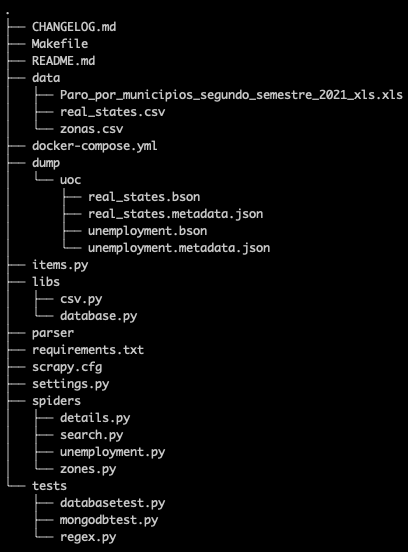
\includegraphics[width=0.7\linewidth]{img/screenshot025}
	\caption{Estructura de directorios del proyecto}
	\label{fig:screenshot025}
\end{figure}

\section{{\itshape Dataset}}

Es una representación en csv de la información volcada en la base de datos NoSQL.


%%%%%%%%%%%%%%%%%%%%%%%%%%%%%%%%%%%%%%%%%%%%%%%%%%%%%%%%%%%%%%%%%%%%%%%
% Referencias
%%%%%%%%%%%%%%%%%%%%%%%%%%%%%%%%%%%%%%%%%%%%%%%%%%%%%%%%%%%%%%%%%%%%%%%
\newpage
\addcontentsline{toc}{section}{Referencias}
\begin{thebibliography}{0}
	
	\bibitem{ciclo} Calvo, M., Pérez, D., Subirats, L. (2019). {\itshape Introducción al ciclo de vida de los datos. } Editorial Universitat Oberta de Catalunya.	
	
	\bibitem{scrap} Subirats, L., Calvo, M. (2019). {\itshape Web Scraping } Editorial Universitat Oberta de Catalunya.
	
	\bibitem{fundamentos} Minguillón, J. (2016). {\itshape Fundamentos de data Science. } Editorial Universitat Oberta de Catalunya.
	
\end{thebibliography}
\end{document}



